\documentclass[14pt, a4paper]{article}
\usepackage[T2A]{fontenc}
\usepackage[utf8]{inputenc}
\usepackage[warn]{mathtext}
\usepackage[english, russian]{babel}
\usepackage{indentfirst}
\usepackage{ncccomma}
\usepackage{color}
\usepackage{amssymb}
\usepackage{amsmath}
\usepackage{graphicx}
\newtheorem{theorem}{Теорема}
\begin{document}



\thispagestyle{empty}
\medskip
\vfill

\begin{center}
\Large{ Конспект лекции по теме \\"Деревья решений. Random forest"\\}
\end{center}

\medskip

\begin{center}
\large{ Небожатко Екатерина}
\end{center}







\newpage
\tableofcontents

\newpage

\section{Бинарное дерево}
Деревом называют конечный связный граф с множеством вершин $V$, не содержащих циклов и имеющий выделенную вершину $v_0 \in V$, в которую не входит ни одно ребро. Эта вершина называется корнем дерева.  Вершина, не имеющая выходящих рёбер, называется терминальной или листом. Остальные вершины называются внутренними. Дерево называется бинарным, если из любой его внутренней вершины выходит ровно два ребра. Выходящие ребра связывают каждую вершину $v$ с левой дочерней вершиной $L_v$ и с правой дочерней $R_v$. 


\section{Постановка задачи}
Решающие деревья применяются для решения сразу двух задач машинного обучения --- задачи классификации и регрессии. 

Пусть дано множество объектов $X$ и множество ответов $Y$. Если Y --- номинальный признак, то мы хотим решить задачу классификации. А именно построить алгоритм $a:X \rightarrow Y$, способный классифицировать произвольный объект $x \in X$. Если Y --- количественный признак, то решаем задачу регрессии: поиск функции $f$, отражающей зависимость 
$y = f(c, x) + \nu$.


\begin{figure}[h!]
\label{fig:class_ex}
\centering
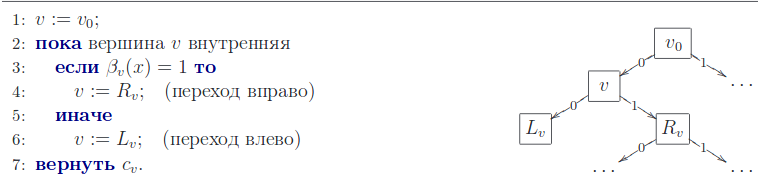
\includegraphics[scale=0.5]{bin_class}
\caption{Классификация объекта $x \in X$ бинарным решающий деревом}
\end{figure}

Пример использования бинарного дерева для классификации \ref{fig:class_ex}.

\section{Регрессионное дерево принятия решений}
Обозначим $X \in \mathbb{R}^{n\times p}$ --- матрицу признаков, $Y \in \mathbb{R^n}$ --- вектор ответов.

Идея построения регрессионного дерева состоит в том, чтобы разделить пространство признаков на $J$ различных, непересекающихся региона $R_1, R_2, \ldots, R_J$. После разбиения, для каждого наблюдения, которое попало в регион $R_j$, мы делаем одинаковые предсказания, равные среднему значению $Y$ в этой области.

Модель задается следующим выражением
\begin{equation}
f(x) = \sum_{j = 1}^J c_j \mathbb{I}(x \in R_j).
\end{equation}

Как мы можем построить регионы $R_1, R_2, \ldots, R_J$? Вообще говоря, области могут быть любой формы, мы выберем прямоугольной, для упрощения интерпретации результатов предсказательной модели. Ищем области, в который RSS минимальна
\begin{equation}
RSS = \sum_{j = 1}^J\sum_{i \in R_j}(y_i - f(x_i))^2.
\end{equation}


Теперь мы можем задать правило выбора $c_j$. 
\begin{equation}
\label{c_solve}
\hat{c_j} = \frac{1}{N_j} \sum_{x_i \in R_j} y_i,
\end{equation}

\noindent где $N_j = \#\{x_i \in R_j \}$.

Конечно, вычислительно не выполнимо перебирать всевозможные разбиения. Алгоритм решения этой задачи, будет представлен ниже.

\section{Дерево классификации}

Пусть теперь $Y$ будет номинативной переменной. Рассмотрим задачу классификации.

Идея построения дерева для задачи классификации очень схожа с задачей регрессии. Мы будем разбивать пространство признаков на непересекающиеся регионы. После разбиения, для каждого наблюдения, которое попало в регион $R_j$, мы делаем предсказание по классу, равное большинству объектов одного класса в этой области. 

Модель задается выражением 
\begin{equation}
p_{jk} = \frac{1}{N_j} \sum_{x_i \in R_j} \mathbb{I}(y_i = k), 
\end{equation}

где $p_{jk}$ --- доля объектов обучающей выборки класса $k$ в $j$том регионе. Будем относить объект в регионе $j$ к классу $k(j) = \arg\max _k p_{jk}$. 

Оптимизационная задача состоит в уменьшении ошибок классификации. Число ошибок классификации --- это просто доля объектов обучающей выборки, которые не относятся к наиболее частому классу в данной области
\begin{equation}
 \frac{1}{N_j} \sum_{x_i \in R_j} \mathbb{I}(y_i \neq  k) = 1 - \max_k(p_{jk}).
\end{equation}

На практике чаще всего используются две другие метрики.

Индекс Джини
\begin{equation}
G = \sum_{k = 1}^K p_{jk}(1 - p_{jk}).
\end{equation}

Кросс-энтропия
\begin{equation}
CI = - \sum_{k = 1}^K p_{jk} \log p_{jk}.
\end{equation}

Эти два индекса численно очень похожи. Они принимают маленькие значения, когда $m$ая вершина содержит элементы преимущественно из одного класса. Они называются информационными.

Индексы представлены на рисунке \ref{fig:index}.

\begin{figure}[h!]
\label{fig:index}
\centering
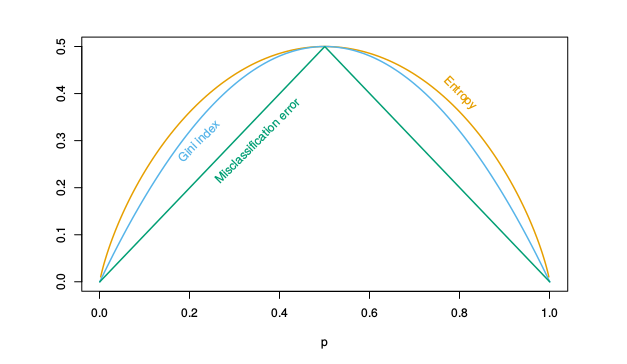
\includegraphics[scale=0.5]{indexes}
\caption{Информационные индексы для 2х классовой классификации, как функция от пропорции $p$ для класса 2.}
\end{figure}

Индекс Джини можно интерпретировать двумя способами. Каждый объект классификации мы можем отнести к классу $k$ $\hat{p}_{jk}$. Значит ошибку классификации мы можем представить в виде $\sum_{k \neq k'} \hat{p}_{jk} \hat{p}_{jk'}$. Также мы можем закодировать каждое наблюдение из класса $k$ как 1, а остальные как 0. Тогда дисперсия в узле для такой переменной будет $\hat{p}_{jk}(1-\hat{p}_{jk})$. Суммируем и получаем индекс Джини.


\section{Алгоритмы}

\subsection{ID3}
Идея алгоритма заключается в последовательном дроблении выборки на две части до тех пор, пока в каждой части не окажутся объекты только одного класса. Проще всего записать этот алгоритм в виде рекурсивной процедуры ID3, которая строит дерево по заданной подвыборке U. Для построения полного дерева она применяется ко всей выборке и возвращает указатель на корень построенного дерева.

\begin{enumerate}
\item Взять все неиспользованные признаки и посчитать их энтропию относительно тестовых образцов;
\item Выбрать признак, для которого энтропия минимальна (а информационная выгода соответственно максимальна);
\item Сделать узел дерева, содержащий этот признак.
\end{enumerate}

\textbf{Формальное описание}
Пусть $U$ --- обучающая выборка, $k$ --- множество значений признаков $Y$.

ID3($U$)
\begin{itemize}
\item Если все $U$ имеют класс $k$, поставить метку 1 в корень и выйти
\item Если ни один объект из $U$ не имеет класс $k$, поставить метку 0 в корень и выйти
\item Выберем предикат $R(x) := \{X| X_j \gtrless s_j \}$ для которого информационная выгода максимальна
\item Разбиваем выборку на две части $U_0$ и $U_1$ по предикату $R$

	$U_0 := \{x \in U: R(x) = 0 \}$;
	
	$U_1 := \{x \in U: R(x) = 1 \}$;
\item Если $U_0 = \varnothing$ или $U_0 = \varnothing$, то создаем новый лист $v$, $k_v$ --- класс, в котором находится большинство объектов из $U$;
\item Иначе создаем новую внутреннюю вершину $v$;

		$R_v$ = $R$

		$L_v$ = ID3$(U_0)$ (создаем левое поддерево)
		
		$R_v$ = ID3$(U_1)$ (создаем правое поддерево)
\end{itemize}

Достоинства:
\begin{itemize}
\item Простота и интерпретируемость классификации.
\item Простота реализации
\end{itemize}

Недостатки:
\begin{itemize}
\item Жадность. Локально оптимальный выбор предиката для разбиения не является глобально оптимальным. В случае неудачного выбора алгоритм не способен вернуться на уровень вверх и заменить неудачный предикат.
\item Высокая чувствительность к составу выборки. Изменение данных в 1–2 объектах часто приводит к радикальному изменению структуры дерева.
\item Алгоритм ID3 переусложняет структуру дерева, и, как следствие, склонен к переобучению.
\end{itemize}

Основная причина недостатков --- неоптимальность жадной стратегии наращивания дерева. Для их устранения применяют различные эвристические приемы: редукцию и построение решающего леса.

\subsection{CART}
Алгоритм CART (Classification and Regression Tree), как видно из названия, решает задачи классификации и регрессии построением дерева решений.

Идея алгоритма 

1. Выберем признак $x_j$ и значение $s_j$, по которой будет происходить разбиение на два региона $R_1$ и $R_2$. Определим их \begin{equation}
\label{region}
 R_1(j,s) = \{x| x_j \leq s_j \} \ \ \ \text{и} \ \ \ R_2(j,s) = \{x| x_j > s_j \}.
 \end{equation}
 Для регрессионного дерева.
 Будем искать значения $s_j$ и $j$, которые являются решением оптимизационной задачи
\begin{equation}
\label{eq:min_split}
\min_{j,s}\left[ \min_{c_1} \sum_{i: x_i \in R_1(j,s)} (y_i - c_1)^2 + \min_{c_2} \sum_{i: x_i \in R_2(j,s)} (y_i - c_2)^2 \right].
\end{equation}

Для любого выбора $j$ и $s_j$ решение \eqref{eq:min_split} есть
\begin{equation}
\hat{c_1} = \frac{1}{N_1} \sum_{x_i \in R_1(j,s_j)} y_i \ \ \ \text{и} \ \ \ \hat{c_2} = \frac{1}{N_2} \sum_{x_i \in R_2(j,s_j)} y_i.
\end{equation}

Перебираем всевозможные значения $s_j$ и выбираем то, которое является оптимальным.

Для дерева классификации выбираем те значения, которые доставляют минимум индексу джини. 

Если $x$ --- номинальная переменная с $l$ категориями, то существует $2^{l-1} -1$ возможных разбиения. Если $x$ --- количественная переменная с $q$ различными значениями, то существует $q-1$ различных вариантов разбиения.

2. Повторяем процесс, разбивая каждый из получившихся регионов, пока не будет достигнут критерий остановки. 

Для выбора оптимального размера дерева используем редукцию.


\subsection{Редукция}
Одна из основных задач состоит в определении оптимального размера дерева. Слишком большое дерево будет переобучаться на тренировочных данных. Слишком маленькое может не содержать достаточной информации о выборочном пространстве.

Суть редукции состоит в удалении поддеревьев, имеющих недостаточную статистическую надёжность. При этом дерево перестаёт
безошибочно классифицировать обучающую выборку, зато качество классификации новых объектов (способность к обобщению), как правило, улучшается.

Рассмотрим одну из возможных эвристик для проведения редукции.

Рассмотрим достаточно большое дерево $T$. Определим поддерево $T_t \subset T$, как любое дерево, которое может быть получено путем образки $T$ в узле $t$.  

Определим функцию cost-complexity 
\begin{equation}
Q_{\alpha}(T) = Q(T) + \alpha |l(T)|,
\end{equation}

\noindent где $Q(T)$ --- training error, $\alpha$ --- настраиваемый параметр, компромисс между размером дерева и его соответствию данным, $l(T)$ --- множество терминальных вершин в дереве $T$.

Для регрессионного дерева
\begin{equation}
Q(T) = \frac{1}{N_j} \sum_{x_i \in R_j} (y_i - \hat{c_j})^2,
\end{equation}

\noindent где $N_j$ и $c_j$ введены в \eqref{c_solve}. 

Для дерева классификации
\begin{equation}
Q(T) = \sum_{t \in l(T)} Q(t),
\end{equation}

сумма ошибочных классификаций в в каждом листе.

Определим изменение cost-complexity функции, при обрезки поддерева $T_t$
\begin{equation}
Q_{\alpha}(T - T_t) - Q_{\alpha}(T) = Q(t) - Q(T_t) + \alpha (1 - |l(T_t)|).
\end{equation}

Пусть $\alpha' = \frac{Q(t) - Q(T_t)}{(|l(T_t)| - 1)}$, тогда изменение cost-complexity функции есть:
\begin{enumerate}
\item 0, когда $\alpha = \alpha'$
\item отрицательно, когда $\alpha < \alpha'$
\item положительно, когда $\alpha > \alpha'$
\end{enumerate}

\textbf{Формальное описание алгоритма}
\begin{enumerate}
\item Пусть $T^1$ дерево полученное при $a^1 = 0$, минимизирующее $Q(T)$
\item Шаг 1. Выберем узел $t \in T^1$, который минимизирует $g_1(t) = \frac{Q(t) - Q(T^1_t)}{(|l(T^1_t)| - 1)}$. Пусть это будет $t_1$,  тогда $\alpha^2 = g_1(t_1)$ и $T^2 = T^1 - T^1_{t_1}$
\item Шаг $i$. Выберем узел $t \in T^i$, который минимизирует $g_i(t) = \frac{Q(t) - Q(T^i_t)}{(|l(T^i_t)| - 1)}$. Пусть это будет $t_i$,  тогда $\alpha^{i+1} = g_i(t_i)$ и $T^{i+1} = T^i - T^i_{t_i}$
\end{enumerate}

В результате работы алгоритма получим последовательность деревьев $T^1 \subset T^2 \subset \ldots \subset \{ root\}$ и последовательность параметров $\alpha^1 \le \alpha^2 \le \ldots \le \alpha^k \le \ldots$.

Выберем $\alpha$ с помощью кросс-валидации и поддерево, соответствующее этому $\alpha$.

Алгоритм просматривает все внутренние вершины дерева и заменяет отдельные вершины либо одной из дочерних вершин (при этом вторая дочерняя удаляется), либо терминальной вершиной. Процесс замен продолжается до тех пор, пока в дереве остаются вершины, удовлетворяющие критерию замены.

Достоинства:
\begin{enumerate}
\item Данный метод является непараметрическим, это значит, что для его применения нет необходимости рассчитывать различные параметры вероятностного распределения.
\item Для применения алгоритма CART нет необходимости заранее выбирать переменные, который будут участвовать в анализе: переменные отбираются непосредственно во время проведения анализа на основании значения индекса Gini.
\item CART легко борется с выбросами: механизм разбиения, заложенный в алгоритме просто помещает выбросы в отдельный узел, что позволяет очистить имеющиеся данные от шумов.
\item Для применения этого алгоритма не надо принимать в расчет никаких предположений или допущений перед проведением анализа.
\item Большим преимуществом является скорость работы алгоритма.
\end{enumerate}

Недостатки:
\begin{enumerate}
\item Деревья решений, предложенные алгоритмом, не являются стабильными: результат, полученный на одной выборке, бывает не воспроизводим на другой (дерево может увеличиваться, уменьшаться, включать другие предикторы и т.д..)
\end{enumerate}

\subsection{Обработка пропусков}
В практических задачах часто возникают пропуски в данных. Самая типичная ситуация, когда значение признака не известно для данного наблюдения, и, следовательно, не определенно значение \eqref{region} в узле. 

1. Стадия обучения. Если значение \eqref{region} не определенно для обучающего объекта $x \in X$, то этот объект не учитывается при вычисления метрик информативности разделения. Соответственно, длина выборки при вычисления информативности уменьшается и критерий должен быть инвариантен относительно длины выборки. Индекс Джини, энтропия и RSS обладают этим свойством.

2. Стадия классификации. Допустим, дерево уже построено, и при классификации нового объекта $x$ значение \eqref{region} во внутренней вершине не определенно. Возможны несколько стратегий обработки этой ситуации. Самая распространенная --- пропорциональное распределение.

\subsection{Оценивание вероятностей}
Во многих приложениях наряду с классификацией объекта $x$ необходимо получать оценки апостериорных вероятностей классов $\hat{P}(y|x)$. Проще всего оценить их как долю обучающих объектов каждого из классов $y \in Y$, попавших в терминальную вершину $v$, классифицировавшую объект $x$ . Однако такая оценка может оказаться смещённой по причине переобучения. Необходимо использовать редукцию и другие подходы для снижения влияния переобучения.

\section{Плюсы и минусы деревьев решений}
\subsection{Дерево решений или линейная модель?}

Деревья решений имеют другой подход к задаче классификации и регрессии, по сравнению с классическим.
Например, модель линейной регрессии имеет вид
\begin{equation}
\label{lr}
f(X)  = \beta_0 + \sum_{j = 1}^pX_j\beta_j.
\end{equation} 

Модель регрессионного дерева имеет вид
\begin{equation}
f(X) = \sum_{m = 1}^M c_m \cdot \mathbb{I}_{(X \in R_m)}.
\end{equation}

Какая из моделей лучше? Если зависимость между признаками и ответом приближенно можно считать линейной, то естественно модель \eqref{lr} будет работать лучше. Если же мы имеем сложную, нелинейную зависимость, то имеет смысл использовать регрессионное дерево. На \ref{fig:treevsLM} представлен пример решения задачи для различной зависимости в данных.

\begin{figure}[h!]
\label{fig:treevsLM}
\centering
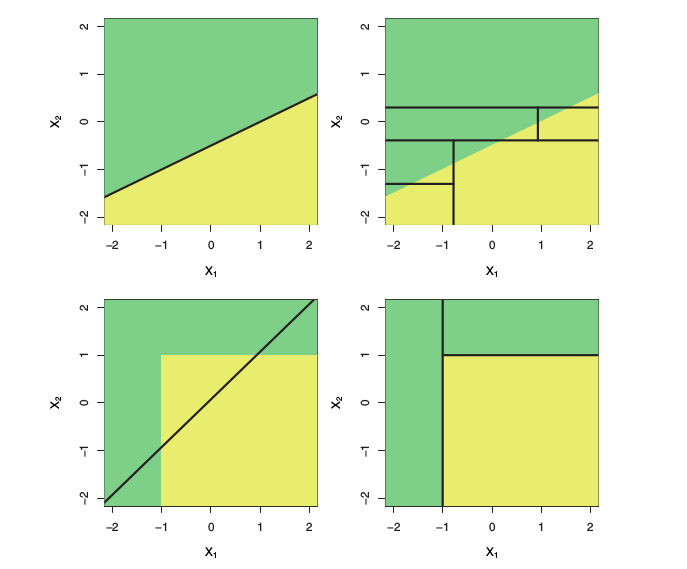
\includegraphics[scale=0.5]{treevsLM}
\caption{Верхняя строка. Пример задачи классификации с линейной зависимостью. Слева решение задачи с помощью классического подхода. Справа решение задачи методом деревьев решений. Нижняя строка. Пример задачи с нелинейной границей. Слева решение регрессией, справа --- дерево решений.}
\end{figure}

\subsection{Преимущества и недостатки деревьев решений}

Преимущества:
\begin{enumerate}
\item Простота интерпретации результатов;
\item Возможность работы как с категориями, так и с количественными значениями;
\item Универсальность в плане решения задач и классификации, и регрессии;
\item Возможность работы с пропусками в данных
\end{enumerate}

Недостатки:
\begin{enumerate}
\item Практическое применение алгоритма деревьев решений основано на эвристических алгоритмах, таких как алгоритм <<жадности>>, где единственно оптимальное решение выбирается локально в каждом узле. Такие алгоритмы не могут обеспечить оптимальность всего дерева в целом;
\item Склонность к переобучению;
\item Метод является неустойчивым. 
\end{enumerate}

\section{Композиция деревьев}
\subsection{Bagging}

Деревья решений, определенные ранее имеют большую вариабильность. В данном контексте это означает, что при построении двух независимых деревьев на одних данным, деревья могут получиться очень разными. Bagging является универсальной процедурой уменьшения вариабельности. 

Рассмотрим независимые одинаково распределенные случайные величины $Z_1, \ldots, Z_n$ c дисперсией $\sigma^2$. Дисперсия среднего $\overline{Z}$ равна $\sigma^2/n$. То есть усреднение величин уменьшает дисперсию. Мы могли бы взять много обучающих выборок из генеральной совокупности, построить для каждой из них предективную модель и усреднить результаты предсказаний. Конечно же, у нас возможности брать множество обучающих выборок. Вместо этого можно использовать идею bootstrap. Будем брать много обучающих выборок из одной, путем равновероятного выбора элементов с повторениями. Такие выборки называются bootsrap sample. Для каждой строим предсказательную модель $f^{*b} (x)$ и усредняем результаты
\begin{equation}
f_{bag}(x) = \frac{1}{B} \sum_{b = 1}^B f^{*b} (x).
\end{equation}

Когда мы говорим о процедуре bagging для задачи классификации, вместо усреднения результатов, можно устраивать голосование среди результатов предсказания и в качестве конечного результата выбирать класс с наибольшим количеством голосов.

Несмотря на то, что результаты bagging обычно лучше, чем результаты одного дерева, при этом теряется один из основных достоинств подхода деревьев решений --- простота интерпретации. Однако мы можем получить информацию о важности каждого и признаков для предсказания. В случае регрессионных деревьев эта величина будет равна общей сумме RSS, которая уменьшилась при разделении, усредненному по всем деревьям. Для деревьев классификации идея аналогичная, только вместо RSS используется индекс джини.

\subsection{Random forest}

Случайный лес (random forest) представляет собой улучшение метода bagging. Как и в bagging, мы строим деревья решений по bootsrap sample, но при этом каждый раз мы выбираем некоторое количество $m$ случайных признаков из всего множества признаков $p$. Обычно полагают $m \approx \sqrt{p}$. На первый взгляд такой подход может показаться странным, однако у него есть разумное объяснение. Предположим, что у нас имеется один признак, который оказывает очень сильное влияние на результат предсказания. При bagging'е почти все деревья будут определяться этим одним признаком, значит будут очень похожи друг на друга. Следовательно, предсказания, полученные методом bagging будут сильно коррелированными. Усреднение коррелированных объектов не приводит к такому же значительному уменьшению дисперсии, как усреднение некоррелированных величин. Случайный лес обходит эту проблему, каждый раз отбирая случайный набор признаков. Мы можем думать об этом, как о процессе декоррелирования деревьев, который позволяет уменьшать дисперсию среднего значения, тем самым повышая его надежность.

\subsection{Почему работают bagging и random forest?}

Ответ на этот вопрос дает теория, связанная с bais-variance decomposition error. Рассмотрим задачу регрессии. 

Пусть $L(y) = (f(x) - y)^2$ --- квадратичная функция потерь. Обозначим метод обучение как $\mu$. Что такое хороший алгоритм? Тот, которого математическое ожидание функции потерь минимально 
$$R(f) = \mathbb{E}_{x,y}(f(x) - y)^2 = \int_x \int_y (f(x) - y)^2 p(x,y) dx dy, $$ где $p(x,y)$ --- плотность совместного распределения $x$ и $y$. $R(f)$ --- среднестатистический риск.

Минимум среднеквадратического риска $f^{*}(x) = \mathbb{E}(y|x) = \int_y y p(y|x) dx$. На практике, конечно, не известны $p(y|x)$ и $p(x,y)$.

Основная мера качества метода обучения $\mu$ 
$$Q(\mu) = \mathbb{E}_{X^l} \mathbb{E}_{x,y}(\mu(X^l)(x) - y).$$

Здесь $\mathbb{E}_{X^l}$ --- математическое ожидание по всевозможным подвыборкам, $\mu(X^l)(x)$ --- применение алгоритма, посчитанного по выборке, к объекту $x$.

\begin{theorem}
В случае квадратичной функции потерь для любого $\mu$
\begin{equation*}
Q(\mu) = \underbrace{\mathbb{E}_{x,y} (f^{*}(x) - y)^2}_{\text{шум}} +  \underbrace{\mathbb{E}_{x,y} (\overline{f}(x) - f^{*}(x))^2}_{\text{смещение}} + \underbrace{ \mathbb{E}_{x,y}\mathbb{E}_{X^l}(\mu(X^l)(x) - \overline{f}(x))^2}_{\text{разброс}},
\end{equation*}
где $\overline{f}(x) = \mathbb{E}_{X^l}(\mu(X^l)(x).$
\end{theorem}

Рассмотрим композицию простого голосования. Пусть $b_t = \mu(X_t^k), X_t^k \sim X^l, t = 1, \ldots, T$ --- обучение алгоритмов по случайным подвыборкам. Обозначим $f_T(x) = \frac{1}{T}\sum_{t=1}^T b_t(x)$ --- композиция простых голосований.

Смещение композиции совпадает со смещением базового алгоритма:
\begin{equation*}
bias = \mathbb{E}_{x,y} (f^{*}(x) -  \mathbb{E}_{X^l}(b_t(x))^2.
\end{equation*}

В bagging строим деревья независимо друг от друга, пытаясь сделать их несмещенными, чтобы они восстанавливали одну и ту же зависимость.

Разброс состоит из дисперсии и ковариации:
\begin{equation*}
variance = \frac{1}{T}\mathbb{E}_{x,y}\mathbb{E}_{X^l}(b_t(x) - \mathbb{E}_{X^l}(b_t(x))^2 + \frac{T-1}{T} \mathbb{E}_{x,y}\mathbb{E}_{X^l}(b_t(x) - \mathbb{E}_{X^l}(b_t(x))(b_s(x) - \mathbb{E}_{X^l}(b_s(x)).
\end{equation*}

Первый член --- это дисперсия одного алгоритма, второй --- ковариация между двумя алгоритмами. 

Выводы:
\begin{enumerate}
\item Bagging уменьшает разброс;
\item Композиции тем менее эффективны, чем сильнее коррелируют базовые алгоритмы;
\item Random forest уменьшает ковариацию базовый алгоритмов.
\end{enumerate}

\subsection{Оценка ошибки Out-of-bag}

Для оценки test error в методах bagging и случайный лес нет необходимости использовать кросс-валидацию. Может быть доказано, что в среднем дерево, построенное на bootsrap sample, использует 2/3 наблюдений. Оставшиеся 1/3 наблюдений будем называть out-of-bag (OOB). Мы можем предсказывать ответ для $i$го наблюдения, использую все деревья, для которых это наблюдение было OOB. Так мы получим B/3 прогнозов для $i$го наблюдения. Для задачи регрессии мы усредним эти прогнозы, а для задачи классификации возьмем наиболее встречающийся класс. Таким образом мы можем получить предсказание OOB для каждого из $n$ наблюдений. Далее может быть посчитана OOB MSE для задачи регрессии или ошибка классификации для задачи классификации. Полученная ошибка OOB является действительной оценкой для модели bagging или случайного леса, поскольку ответ для каждого наблюдения прогнозируется с использованием деревьев, в которых это наблюдение не использовалось. Для достаточно больших $B$, ошибка OOB будет практически эквивалентна k-слойной ошибки кросс-валидации. OOB подход используют для данных большого объема, когда кросс-валидацию провести вычислительно трудно.



\end{document}